\usection{Modelica}

\lstset{frame=tb,
language=modelica,
aboveskip=3mm,
belowskip=3mm,
showstringspaces=false,
columns=flexible,
basicstyle={\small\ttfamily},
numbers=none,
numberstyle=\tiny\color{gray},
keywordstyle=\color{blue},
commentstyle=\color{dkgreen},
stringstyle=\color{mauve},
breaklines=true,
breakatwhitespace=true,
tabsize=2
}

\begin{figure}[H]
  \centering
  \begin{circuitikz}[american voltages, american currents, scale = 0.75]
    \draw
    (0, 0)
    to [battery=$V(t)$] (0, 2)
    to [open, v=$ $] (0, 0) to [open] (0, 4)
    to [switch, mirror] (0, 2) to [open] (0, 4)
    to [R=$R$] (4, 4)
    to [L=$L$] (4, 0)
    to [C=$C$] (0, 0)
    ;
  \end{circuitikz}
  \caption{Modelo gráfico.}
\end{figure}

\usubsection{Caso General}

Cuando el interruptor está cerrado se tiene:
\begin{equation*}
  V(t) = Ri(t) + L\frac{di(t)}{dt} + \frac{1}{C}\int_{0}^ti(t)dt
\end{equation*}

Se aplica la transformada de Laplace:
\begin{align*}
  V(s) &= RI(s)
  + L \left[ sI(s) - i(0) \right]
  + \frac{1}{C} \left[ \frac{1}{s} I(s) \right] \nonumber
  = I(s) \left[R + Ls +\frac{1}{Cs}\right] - Li(0)
\end{align*}
\begin{align*}
  I(s) &= \frac{V(s) + Li(0)}{Ls^2 + Rs + \frac{1}{C}}
  = \frac{L\left(V(s) + Li(0)\right)}{s^2 + \frac{R}{L}s + \frac{1}{LC}}
\end{align*}
\begin{align*}
  s_1 &= \frac{-\frac{R}{L} - \sqrt{\left(\frac{R}{L}\right)^2-\frac{4}{LC}}}{2}
  &
  s_2 &= \frac{-\frac{R}{L} + \sqrt{\left(\frac{R}{L}\right)^2-\frac{4}{LC}}}{2}
\end{align*}
\begin{equation*}
  I(s) = \frac{L\left(V(s) + Li(0)\right)}{(s-s_1)(s-s_2)}
  = \frac{A}{s-s_1} + \frac{B}{s-s_2}
\end{equation*}
\begin{align*}
  L\left(V(s) + Li(0)\right) = A(s-s_2) + B(s-s_1)
\end{align*}
\begin{align*}
  A &= \frac{L\left(V(s_1) + Li(0)\right)}{s_1-s_2}
  &
  B &= \frac{L\left(V(s_2) + Li(0)\right)}{s_2-s_1}
\end{align*}
\begin{align*}
  I(s) &= \frac{L\left(V(s_1) + Li(0)\right)}{s_1-s_2}\frac{1}{s-s_1} +
  \frac{L\left(V(s_2) + Li(0)\right)}{s_2-s_1}\frac{1}{s-s_2}
\end{align*}

Se aplica la transformada inversa de Laplace:

\begin{align*}
  i(t) &=
  \frac{L\left(V(s_1) + Li(0)\right)}{s_1-s_2}e^{s_1t} +
  \frac{L\left(V(s_2) + Li(0)\right)}{s_2-s_1}e^{s_2t}
\end{align*}

\usubsection{Caso 1}

\usubsubsection{Solución Teórica}

\begin{align*}
  R&=4k\Omega&
  C&=75\mu F&
  L&=2mH
\end{align*}
\begin{align*}
  s_1 &= \frac{-\frac{4k\Omega}{2mH}
  - \sqrt{\left(\frac{4k\Omega}{2mH}\right)^2-\frac{4}{2mH75\mu F}}}{2}
  &
  s_2 &= \frac{-\frac{4k\Omega}{2mH}
  + \sqrt{\left(\frac{4k\Omega}{2mH}\right)^2-\frac{4}{2mH75\mu F}}}{2}
\end{align*}

\usubsubsection{Simulación}

\begin{figure}[H]
  \lstinputlisting{modelica/RLCSerie1.mo}
  \caption{Código para el primer caso.}
\end{figure}

\begin{figure}[H]
  \centering
  \label{gr:caso1:corrientes}
  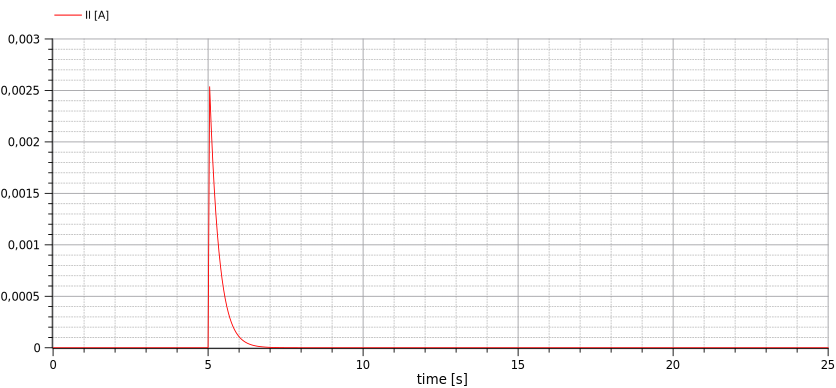
\includegraphics[width=\textwidth]{modelica/graficas/1-corrientes}
  \caption{Gráfica de Corrientes para el primer caso.}
\end{figure}

\begin{figure}[H]
  \centering
  \label{gr:caso1:tensiones}
  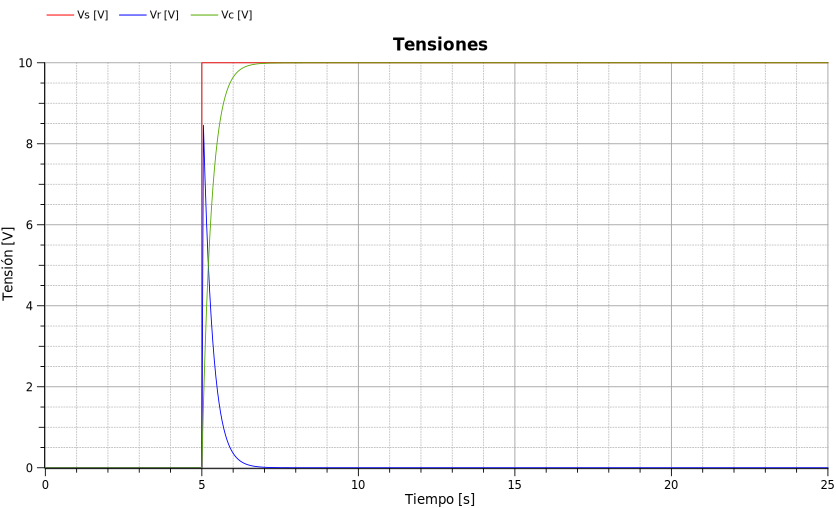
\includegraphics[width=\textwidth]{modelica/graficas/1-tensiones}
  \caption{Gráfica de Tensiones para el primer caso.}
\end{figure}

\usubsection{Caso 2}

\usubsubsection{Solución Teórica}

\begin{align*}
  R&=20k\Omega&
  C&=100\mu F&
  L&=7mH
\end{align*}
\begin{align*}
  s_1 &= \frac{-\frac{20k\Omega}{7mH}
  - \sqrt{\left(\frac{20k\Omega}{7mH}\right)^2-\frac{4}{7mH100\mu F}}}{2}
  &
  s_2 &= \frac{-\frac{20k\Omega}{7mH}
  + \sqrt{\left(\frac{20k\Omega}{7mH}\right)^2-\frac{4}{7mH100\mu F}}}{2}
\end{align*}

\usubsubsection{Simulación}

\begin{figure}[H]
  \begin{lstlisting}
    model RLCSerie2
      import Modelica.SIunits.Resistance;
      import Modelica.SIunits.Capacitance;
      import Modelica.SIunits.Inductance;
      import Modelica.SIunits.Voltage;
      import Modelica.SIunits.Current;

      parameter Resistance R = 20000.0;
      parameter Capacitance C = 0.000100;
      parameter Inductance L = 0.007;

      Voltage Vs, Vr, Vl;
      Voltage Vc(start=0, fixed=true);
      Current Il(start=0, fixed=true);

    equation
      Vs = if time >= 5.0 then 10 else 0;
      Vr = R * Il;
      Vl = L * der(Il);
      Il = C * der(Vc);
      Vs = Vr + Vl + Vc;
      annotation(experiment(StartTime=0.0, StopTime=25.0));
    end RLCSerie2;
  \end{lstlisting}
  \caption{Código para el segundo caso.}
\end{figure}

\begin{figure}[H]
  \centering
  \label{gr:caso1:corrientes}
  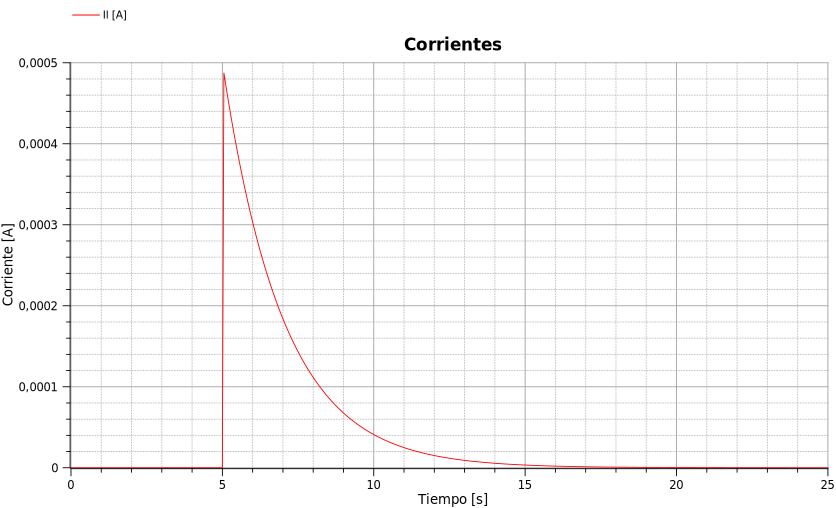
\includegraphics[width=\textwidth]{modelica/graficas/2-corrientes}
  \caption{Gráfica de Corrientes para el segundo caso.}
\end{figure}

\begin{figure}[H]
  \centering
  \label{gr:caso1:tensiones}
  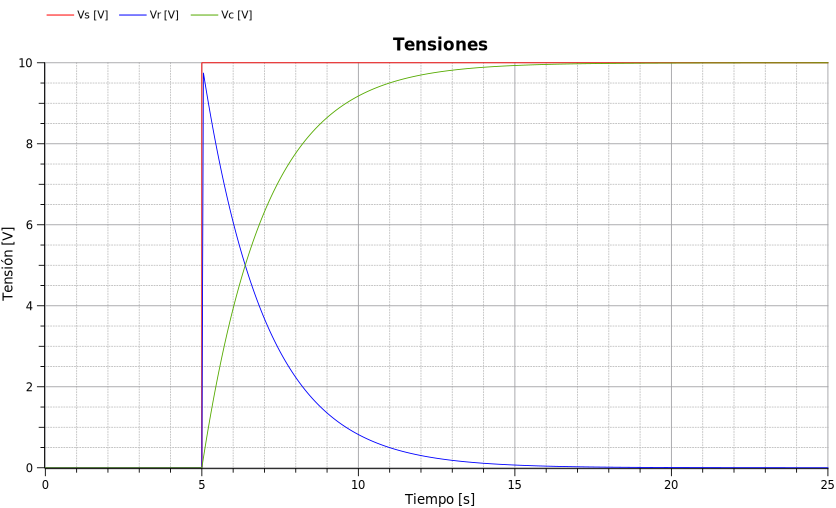
\includegraphics[width=\textwidth]{modelica/graficas/2-tensiones}
  \caption{Gráfica de Tensiones para el segundo caso.}
\end{figure}

\usubsection{Caso 3}

\usubsubsection{Solución Teórica}

\begin{align*}
  R&=5k\Omega&
  C&=470\mu F&
  L&=5mH
\end{align*}
En este caso $t_0=0$.
\begin{align*}
  s_1 &= \frac{-\frac{5k\Omega}{5mH}
  - \sqrt{\left(\frac{5k\Omega}{5mH}\right)^2-\frac{4}{5mH470\mu F}}}{2}
  &
  s_2 &= \frac{-\frac{5k\Omega}{5mH}
  + \sqrt{\left(\frac{5k\Omega}{5mH}\right)^2-\frac{4}{5mH470\mu F}}}{2}
\end{align*}

\usubsubsection{Simulación}

\begin{figure}[H]
  \begin{lstlisting}
    model RLCSerie3
      import Modelica.SIunits.Resistance;
      import Modelica.SIunits.Capacitance;
      import Modelica.SIunits.Inductance;
      import Modelica.SIunits.Voltage;
      import Modelica.SIunits.Current;

      parameter Resistance R = 5000.0;
      parameter Capacitance C = 0.000470;
      parameter Inductance L = 0.005;

      Voltage Vs, Vr, Vl;
      Voltage Vc(start=0, fixed=true);
      Current Il(start=0, fixed=true);

    equation
      Vs = if (time >= 5.0 and time <= 7.0) or (time >= 15) then 10 else 0;
      Vr = R * Il;
      Vl = L * der(Il);
      Il = C * der(Vc);
      Vs = Vr + Vl + Vc;
      annotation(experiment(StartTime=0.0, StopTime=25.0));
    end RLCSerie3;
  \end{lstlisting}
  \caption{Código para el tercer caso.}
\end{figure}

\begin{figure}[H]
  \centering
  \label{gr:caso1:corrientes}
  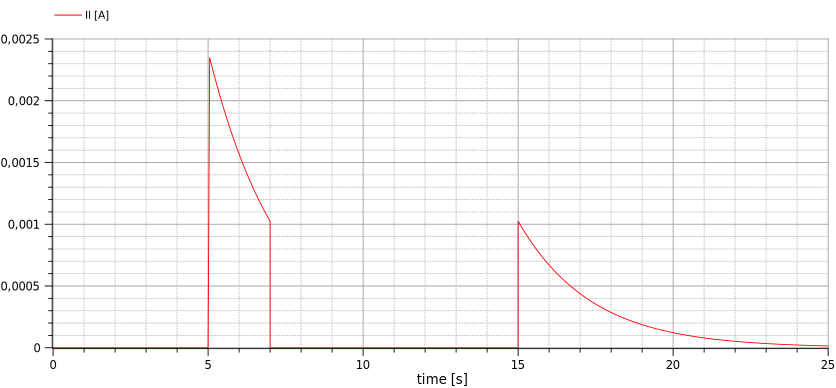
\includegraphics[width=\textwidth]{modelica/graficas/3-corrientes}
  \caption{Gráfica de Corrientes para el tercer caso.}
\end{figure}

\begin{figure}[H]
  \centering
  \label{gr:caso1:tensiones}
  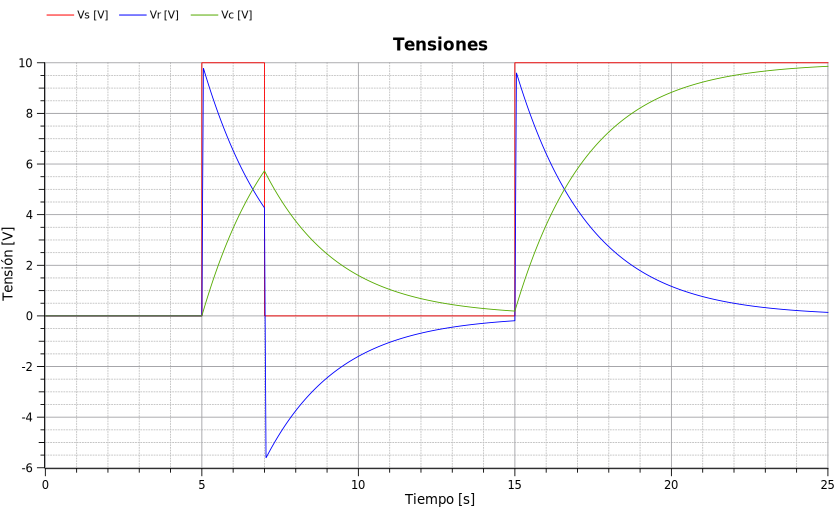
\includegraphics[width=\textwidth]{modelica/graficas/3-tensiones}
  \caption{Gráfica de Tensiones para el tercer caso.}
\end{figure}

